\documentclass{ximera}

\graphicspath{{./content/02_8_more_tnb/graphics/}{./graphics/}}

\title{Moving Frame Computations}
\begin{document}
\begin{abstract}
\end{abstract}
\maketitle

Recall our definition of the moving frame:

\begin{definition}
Given a path $\vec{x}(t)$, we define the \emph{moving frame} of the path to be the triple $(\vec{T},\vec{N},\vec{B})$.

$\vec{T}$ is the \emph{unit tangent vector},
\[
\vec{T}(t) = \dfrac{\vec{x}'(t)}{\|\vec{x}'(t)\|}.
\]

$\vec{N}$ is the \emph{unit normal vector},
\[
\vec{N}(t) = \dfrac{\vec{T}'(t)}{\|\vec{T}'(t)\|}.
\]

$\vec{B}$ is the \emph{unit binormal vector},
\[
\vec{B}(t) = \vec{T}(t)\times\vec{N}(t).
\] 

The moving frame is also called the \emph{TNB frame}.
\end{definition}

We'll now work through some moving frame computations. These computations can sometimes get quite nasty, so it's important to simplify as you go, and plug in points when possible.

\section*{Examples}

\begin{example}
We'll compute the moving frame for the path $\vec{x}(t) = (\cos(t),\sin(t), t)$ in general, and when $t = 0$.

In order to find the unit tangent vector, we first need to find the velocity vector.
\[
\vec{x}'(t) = \answer{(-\sin(t), \cos(t), 1)}
\]
Computing the length, we have
\[
\|\vec{x}'(t)\| = \answer{\sqrt{2}}.
\]
From these, we compute
\begin{align*}
\vec{T}(t) &= \dfrac{\vec{x}'(t)}{\|\vec{x}'(t)\|}\\
&= \answer{(-\frac{1}{\sqrt{2}}\sin(t), \frac{1}{\sqrt{2}}\cos(t), \frac{1}{\sqrt{2}})}.
\end{align*}
Plugging in $t=0$, we have
\[
\vec{T}(0) = \answer{(0,\frac{1}{\sqrt{2}},\frac{1}{\sqrt{2}})}.
\]
Next, we need to find the unit binormal vector. For this, we first need to find $\vec{T}'(t)$.
\[
\vec{T}'(t) = \answer{(-\frac{1}{\sqrt{2}}\cos(t), -\frac{1}{\sqrt{2}}\sin(t), 0)}
\]
Computing the length, we have
\[
\|\vec{T}'(t)\| = \answer{\frac{1}{\sqrt{2}}}.
\]
From these, we compute
\begin{align*}
\vec{N}(t) &= \dfrac{\vec{T}'(t)}{\|\vec{T}'(t)\|}\\
&= \answer{(-\cos(t), -\sin(t),0)}.
\end{align*}
Plugging in $t=0$, we have
\[
\vec{N}(t) = \answer{(-1,0,0)}.
\]
Finally, we need to find the unit binormal vector.
\begin{align*}
\vec{B}(t) &= \vec{T}(t)\times\vec{N}(t)\\
&= \answer{(\frac{1}{\sqrt{2}}\sin(t), -\frac{1}{\sqrt{2}}\cos(t), \frac{1}{\sqrt{2}})}
\end{align*}
Plugging in $t=0$, we have
\[
\vec{B}(0) = \answer{(0, \frac{1}{\sqrt{2}}, \frac{1}{\sqrt{2}})}.
\]

\youtube{youtu.be/230jX21EO3A}

\end{example}

\begin{example}
We'll compute the moving frame for the path $\vec{x}(t) = (1, t, t^2)$ when $t=1$.

Since we only need the moving frame for one specific value of $t$, we'll plug in this value as soon as we can, to help simplify computation. However, we need to make sure that we've taken all necessary derivatives before plugging in $t=1$.

In order to find the unit tangent vector, we first need to find the velocity vector.
\[
\vec{x}'(t) = \answer{(0, 1, 2t)}
\]
If we only needed to find $\vec{T}(1)$, we could plug in $t=1$ at this point. However, we will eventually need to differentiate $\vec{T}(t)$ to find $\vec{N}(t)$, so we'll hold off on plugging in $t=1$ for now.

Next, we find the length of $\vec{x}'(t)$.
\[
\|\vec{x}'(t)\| = \answer{\sqrt{1+4t^2}}
\]

Then, we have that the unit tangent vector is
\begin{align*}
\vec{T}(t) &= \dfrac{\vec{x}'(t)}{\|\vec{x}'(t)\|}\\
&= \answer{(0,\frac{1}{\sqrt{1+4t^2}}, \frac{2t}{\sqrt{1+4t^2}})}.
\end{align*}

Plugging in $t=1$, we have
\[
\vec{T}(1) = \answer{(0,\frac{1}{\sqrt{5}}, \frac{2}{\sqrt{5}})}.
\]

Next, we differentiate $\vec{T}(t)$. Take a moment to revel in gratitude that we're doing this computation for you.
\[
\vec{T}'(t) = \left(0,\frac{-4t}{(1+4t^2)^{3/2}}, \frac{2}{(1+4t^2)^{3/2}}\right)
\]
At this point, we don't have anymore derivatives to take, so we'll plug in $t=1$ before continuing our computation.
\[
\vec{T}'(1) = \answer{(0,\frac{-4}{5^{3/2}}, \frac{2}{5^{3/2}})}
\]
The length of this vector is
\[
\|\vec{T}'(1)\| = \answer{2/5}.
\]
From these, we compute the unit normal vector when $t=1$,
\begin{align*}
\vec{N}(1) &= \dfrac{\vec{T}'(1)}{\|\vec{T}'(1)\|}\\
&= \answer{(0,\frac{-2}{\sqrt{5}},\frac{1}{\sqrt{5}})}.
\end{align*}
Finally, we compute the unit binormal vector when $t=1$.
\begin{align*}
\vec{B}(1) &= \vec{T}(1)\times\vec{N}(1)\\
&= \answer{(1,0,0)}
\end{align*}
Notice how helpful it was to plug in $t=1$ as early as we could!

\begin{image}
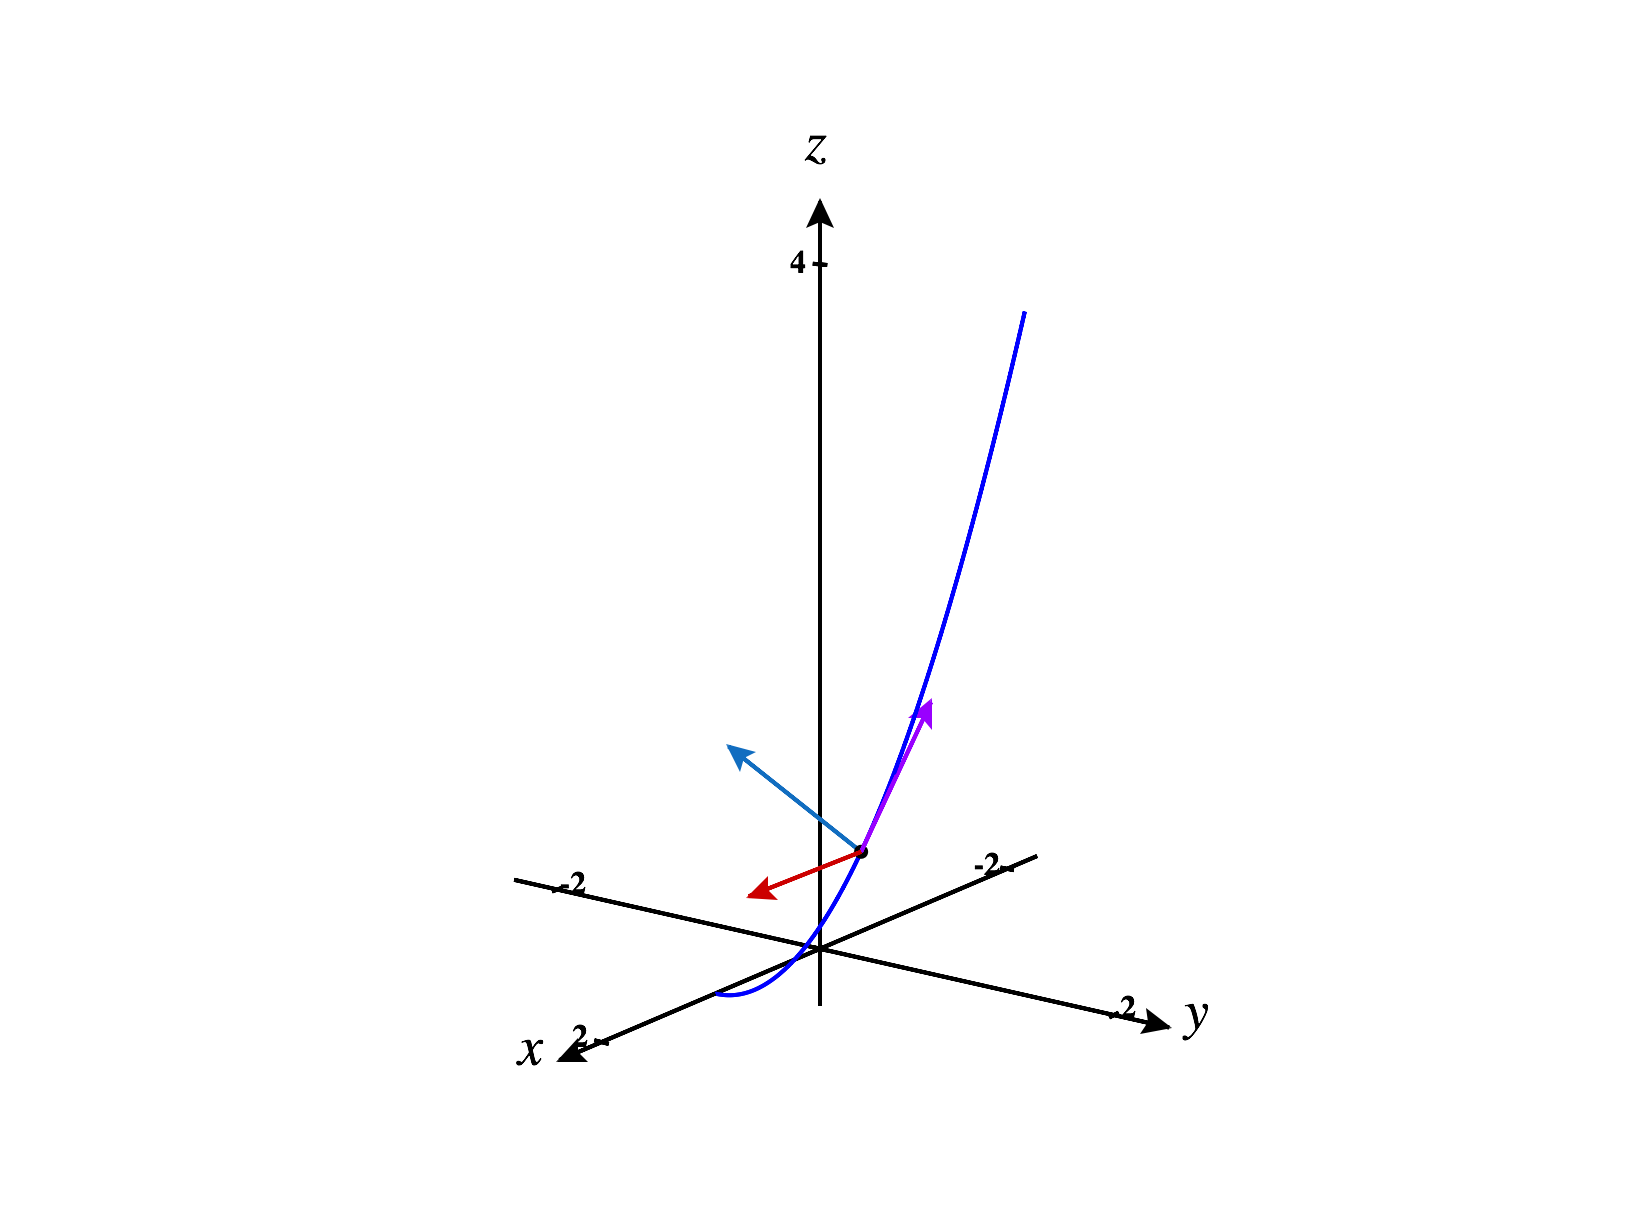
\includegraphics[width = \textwidth]{CalcPlot3D-tnb_parabola}
\end{image}
\end{example}

\textit{Images were generated using \href{https://www.monroecc.edu/faculty/paulseeburger/calcnsf/CalcPlot3D/}{CalcPlot3D}.}

\end{document}